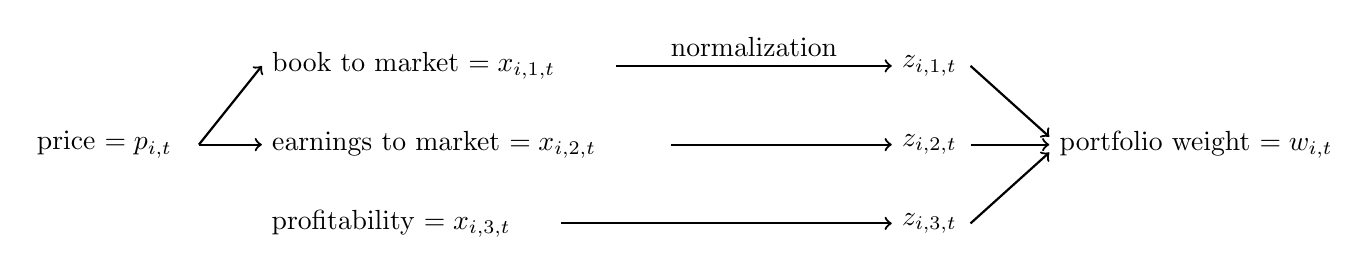
\begin{tikzpicture}
\node[text centered] at (0,0) {price $= p_{i,t}$};
\draw[->,thick] (1.2, 0) -- (2, 1) node [right] {book to market $= x_{i,1,t}$};
\draw[->,thick] (1.2, 0) -- (2, 0) node [right] {earnings to market $= x_{i,2,t}$};
\node[align=left] at (2,-1) [right] {profitability $= x_{i,3,t}$};
%\draw[->, thick] (1.2, 0) -- (2, -1);
%\node[text centered, red, rotate=135] at (1.6, -0.5) {\large X};
\draw[->,thick] (6.5, 1) -- (10, 1) node [right] {$z_{i,1,t}$};
\node[text centered, above] at (8.25, 1) {normalization};
\draw[->,thick] (7.2, 0) -- (10, 0) node [right] {$z_{i,2,t}$};
\draw[->,thick] (5.8, -1) -- (10, -1) node [right] {$z_{i,3,t}$};
\draw[->,thick] (11, 1) -- (12, 0.1);
\draw[->,thick] (11, 0) -- (12, 0) node [right] {portfolio weight $= w_{i,t}$};
\draw[->,thick] (11, -1) -- (12, -0.1);
\end{tikzpicture}